\section{Results Discussion}
\label{sec:discussion}


Figure~\ref{fig:overall} illustrates the performance, energy, and the
energy-delay (ED) product  of the OoO and BB cores normalized to the InO
processor.  On average, BB closes 61\% of the performance gap between INO and
OoO while closing 65\% of their energy gap. Overall, the energy delay product of
BB is 24\% more effective than InO and 21\% more effective than OoO.
\begin{figure*}[h]
	\centering
	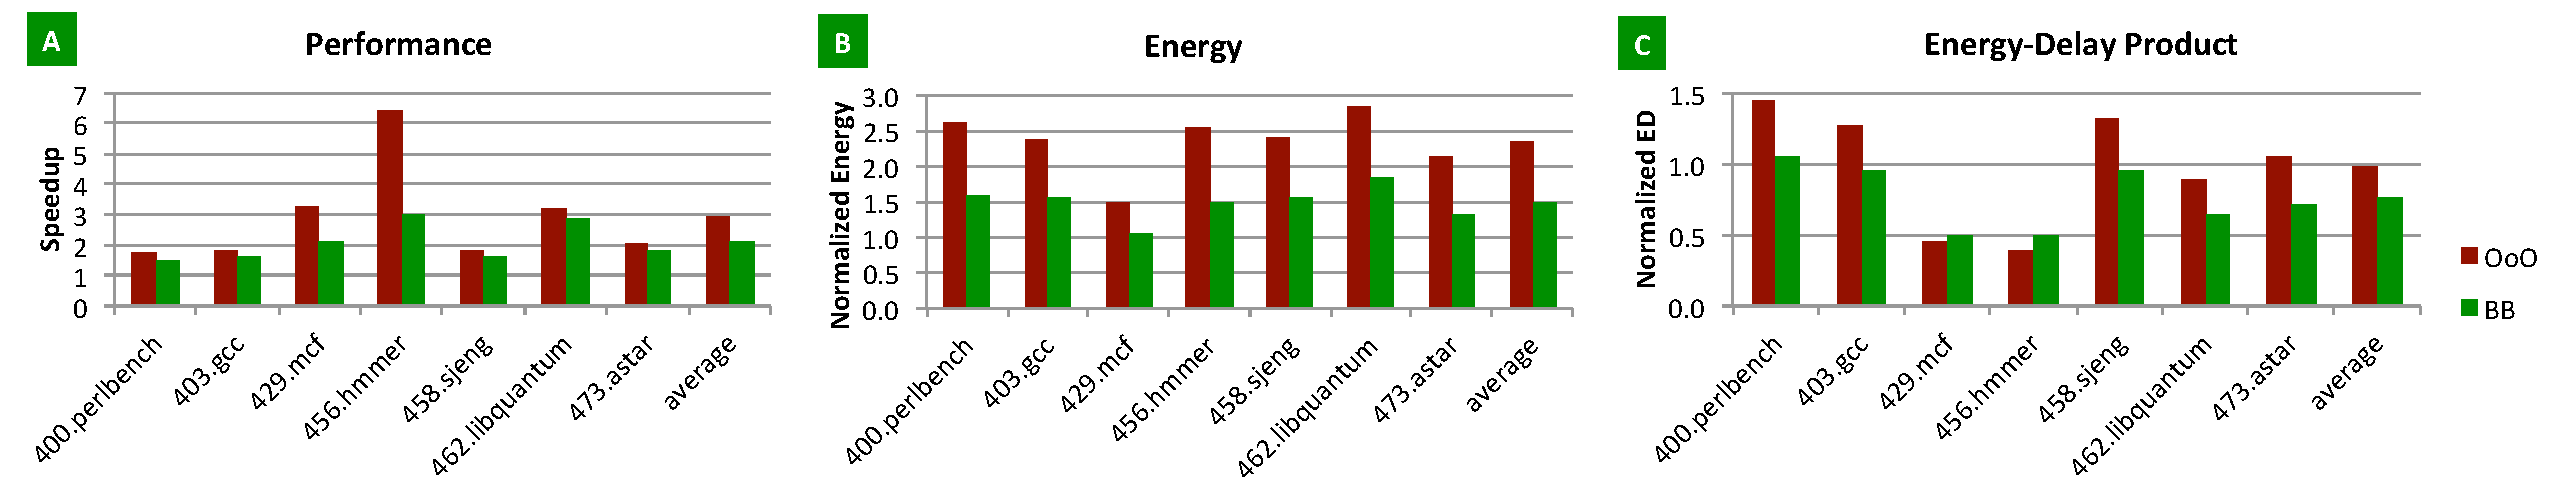
\includegraphics[width=\textwidth]{result/overall_perf.pdf} 
    \caption{(A) $IPC_{CORE}/IPC_{BASE}$, (B) $E_{CORE}/E_{BASE}$, (C)
        $ED_{CORE}/ED_{BASE}$; $CORE$ refers to BB and OoO and $BASE$ refers to
            INO core.}
	\label{fig:overall}
\end{figure*}

Figure~\ref{fig:ep} illustrates the energy versus performance plot for the three
processors when using 2-wide, 4-wide, and 8-wide architectures. Each point on
the figure is the average (speedup, energy) of SPEC benchmarks evaluated here.
While OoO provides best performance, we see the BB architecture with 8
functional units is at the lowest right corner of the graph, making it the best
design choice. Comparing Figure~\ref{fig:ep} with Figure~\ref{fig:insight} shows
the effect of the BB architecture in pushing the trend towards the more energy
efficient corner. There is still more work to be done to push the performance
point of BB further to the right.
\begin{figure}[!htbp]
	\centering
	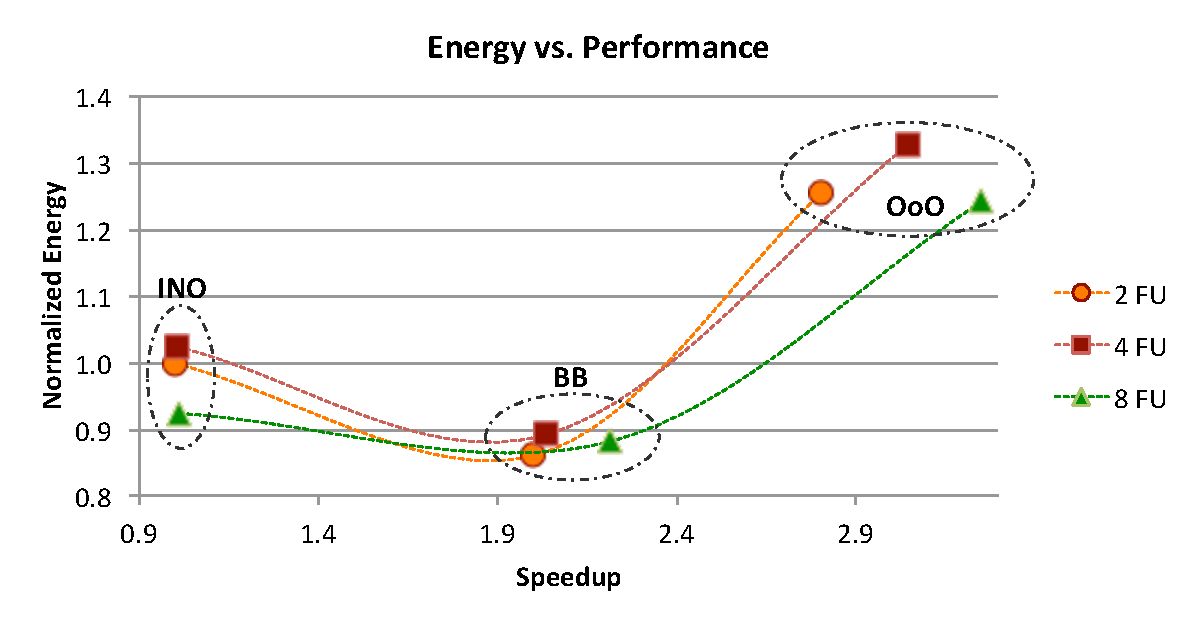
\includegraphics[width=1.0\columnwidth]{result/ep.pdf} 
    \caption{Energy vs. Performance Trend for OoO, BB, \& InO}
	\label{fig:ep}
\end{figure}

Figure~\ref{fig:bbWin_size} illustrates the change in performance and energy of
BB when the BB Window size changes. Recall that the number of available FIFO
slots in these buffers define how the compiler partitions basic-blocks. The
smaller the FIFO size, the more fine grain the code, the more the number of BB's
in-flight to issue instructions. Overall, we observe 15\% average performance
drop and XX\% energy gain when BB Window size changes from 5 to 15 entries.
\begin{figure}[!htbp]
	\centering
	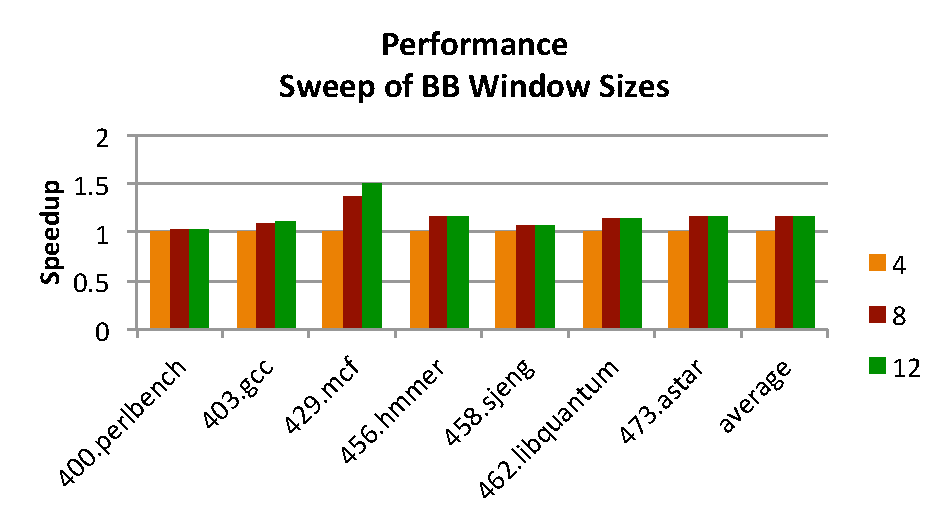
\includegraphics[width=1.0\columnwidth]{result/bbWin_size.pdf} 
    \caption{Performance \& energy change with sweeping the BB Window FIFO queue size}
	\label{fig:bbWin_size}
\end{figure}

Figure~\ref{fig:bbWin_ins_cnt} evaluates the effect of BB Window count on the
performance of BB architectures. We observe 16\% speedup gain between 4 and 8
instruction BB Windows, but not so much beyond. This result suggests  eight BB
Windows are sufficient to get optimum performance gains while keeping the energy
at a relatively low value. Because gcc has small basic-blocks with independent
instructions, it makes best use of the extra BB Window resources to improve the
ILP by up to 50\% while saving up to 8\% in energy as a result.
\begin{figure}[!htbp]
	\centering
	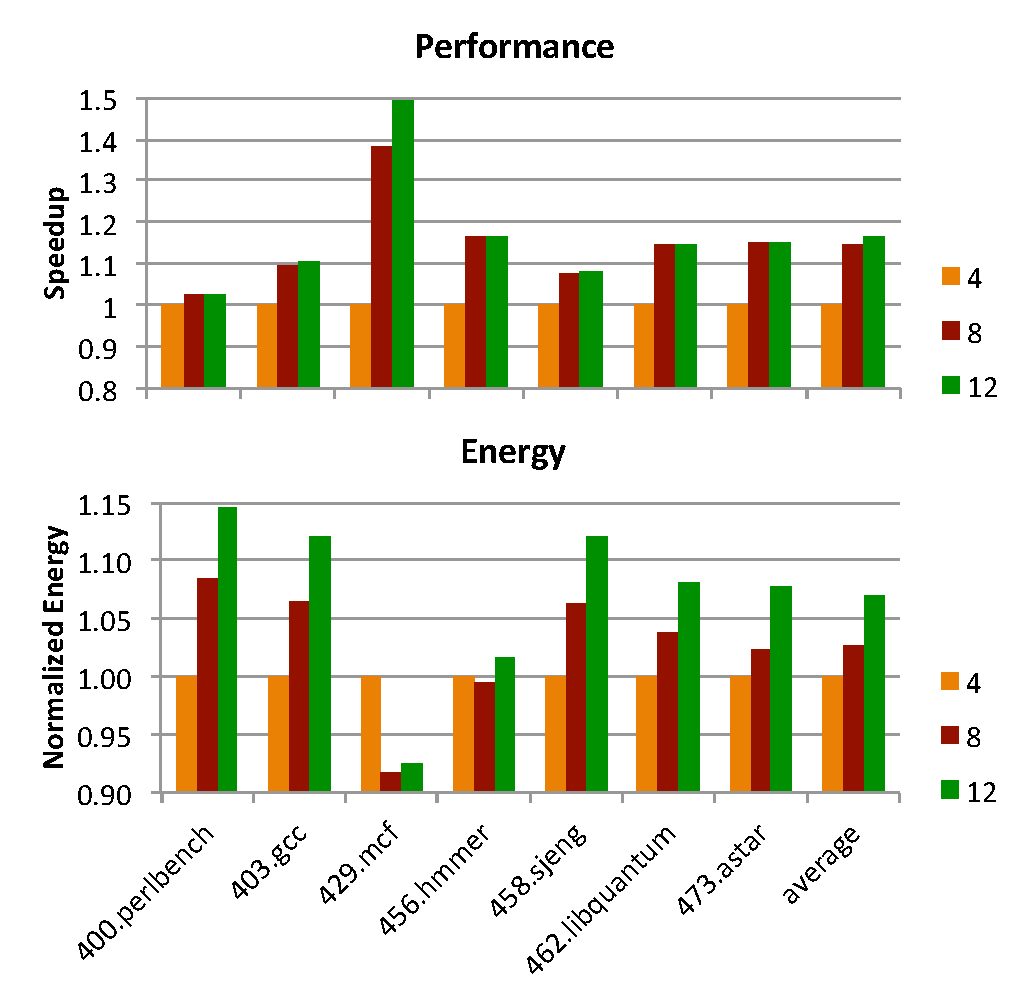
\includegraphics[width=1.0\columnwidth]{result/bbWin_ins_cnt.pdf} 
    \caption{Performance \& energy change with sweeping the number of BB Windows}
	\label{fig:bbWin_ins_cnt}
\end{figure}

Figure~\ref{fig:bbWin_port} evaluates the performance improvement trend as the
number of read ports for BB Windows increase from 1 to 8 ports. While eight
ports provides 11\% average performance gains, three ports provides 10\%.  Given
the XX\% energy overhead of 8-ported BBWindows, we find three read ports the
optimal port count for achieving optimal ED product.
\begin{figure}[!htbp]
	\centering
	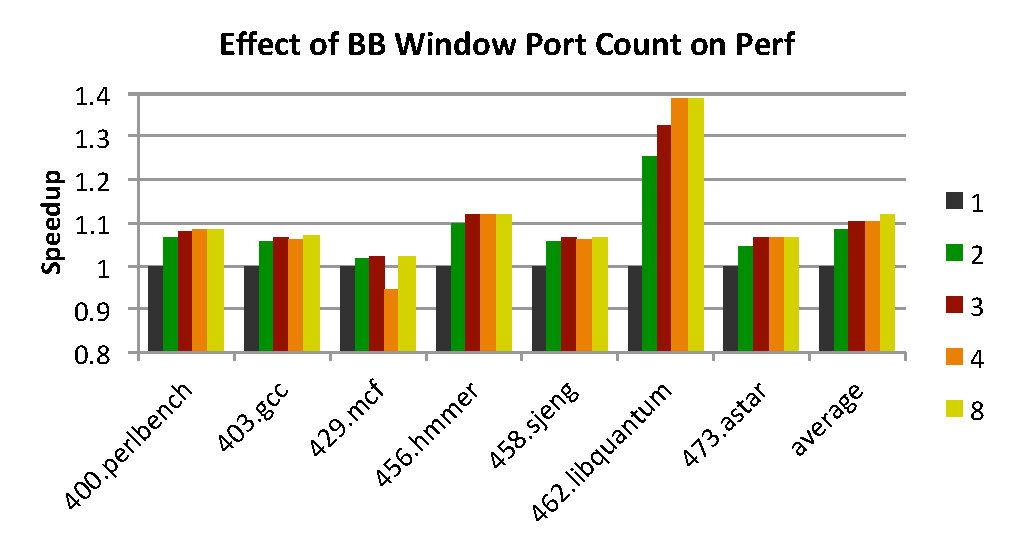
\includegraphics[width=1.0\columnwidth]{result/bbWin_port.pdf} 
    \caption{Performance \& energy change with sweeping the number of BB Window
    ports}
	\label{fig:bbWin_port}
\end{figure}

Figure~\ref{fig:lrf_effect} shows 12\% average increase in speedup and 19\%
reduction in energy consumption of BBE when the register allocator uses LRF
versus when it only uses the global register file for all operations.
\begin{figure}[!htbp]
	\centering
	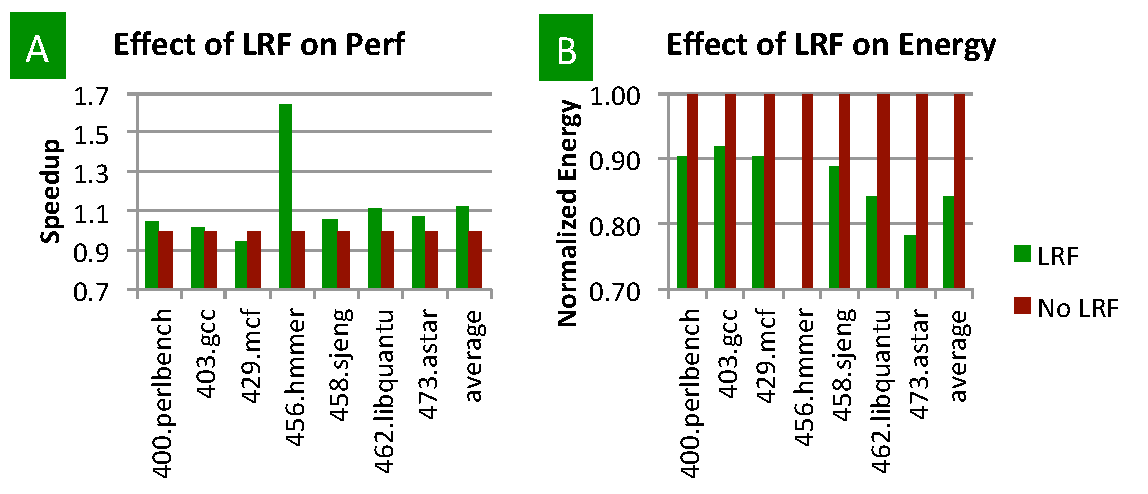
\includegraphics[width=1.0\columnwidth]{result/lrf_effect.pdf} 
    \caption{Performance \& energy change with sweeping the number of BB Windows}
	\label{fig:lrf_effect}
\end{figure}


As mentioned earlier in the paper, BBE benefits from optimal basic-block
instructions scheduling, making each basic-block issue instructions at the
highest issue rate possible. This implies enabling the scheduler to identify
data dependency chains in the code and scheduling instructions such that they
can be issued back-to-back while using the common data-bus for reading their
input operands. Figure~\ref{fig:forwarding} shows BB is 39\% more effective in
leveraging data-forwarding while issuing instructions. The bar charts are
normalize to the forwarding ability of the InO core. 
\begin{figure}[!htbp]
	\centering
	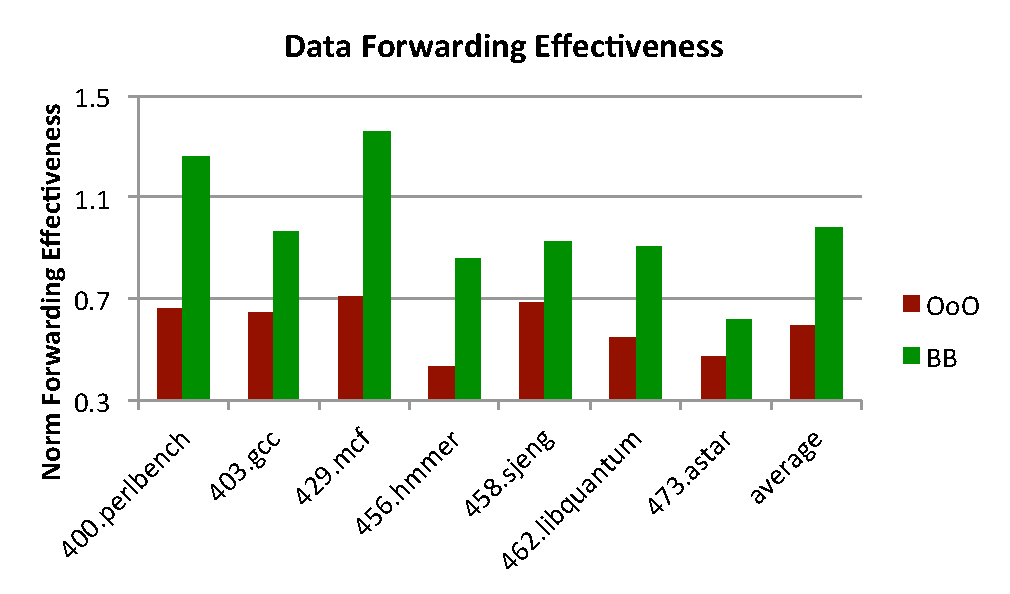
\includegraphics[width=1.0\columnwidth]{result/forwarding.pdf} 
    \caption{Energy vs. Performance Trend for OoO, BB, \& InO}
	\label{fig:forwarding}
\end{figure}

As mentioned in Section~\ref{sec:bpu}, the BB core reduces the number branch
lookup accesses to the branch prediction unit, including the BTB.
Figure~\ref{fig:bpu} illustrates, on average, BB looks up the BPU 35\% less
frequently, making it just as much more energy efficient than OoO.
\begin{figure}[!htbp]
	\centering
	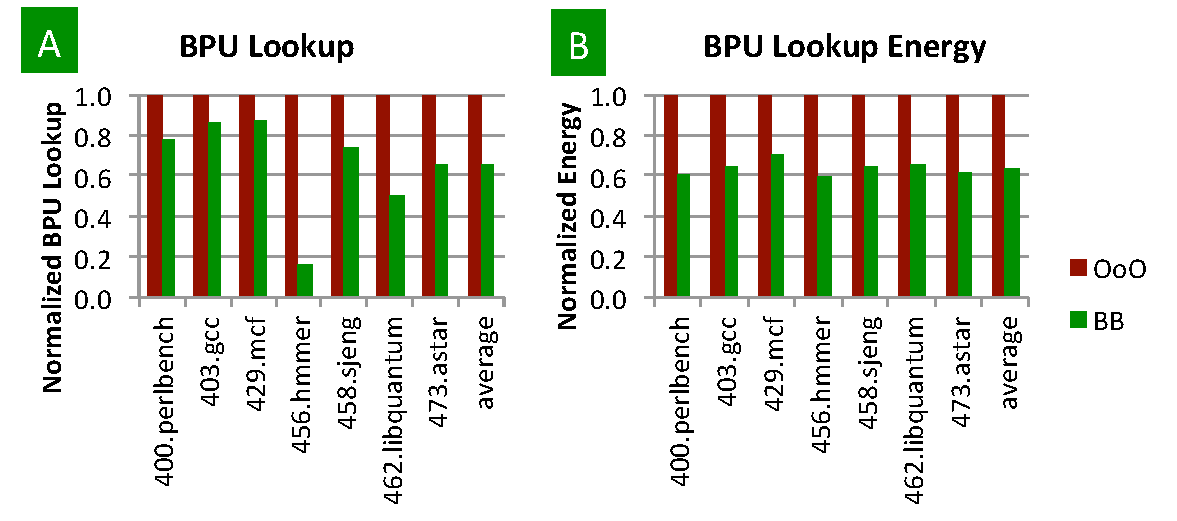
\includegraphics[width=1.0\columnwidth]{result/bpu.pdf} 
    \caption{(A) Normalized ratio of BPU accesses by BBE wrt. OoO. (B)
        Normalized lookup energy reduction ratio of BB wrt. OoO.}
	\label{fig:bpu}
\end{figure}


area evaluation.

%evaluation of pipeline stages.
%comparison of new and conventional register rename model.
%comparison of new and conventional squash mode.
%sweep of register file sizes. 


